\chapter{Day 5: LSAE, Brain data, and C\&E}

\section{Schedule}
\begin{itemize}
    \item 0900-0915: Table Dynamics Discussion
    \item 0915-1010: Debrief and Synthesis
    \item 1010-1025: Coffee Break
    \item 1025-1035: Correlation
    \item 1035-1135: Brain Data with Samantha Michalka!
    \item 1135-1220: AI and Society Discussion
    \item 1220-1230: Day Survey
\end{itemize}

\section{Table Dynamics Survey Discussion}

\section{Debrief and Synthesis}

\bi
\item Please discuss your overnight work with your table-mates, and get help with the ideas that you are still confused by.
\ei

In the next set of exercises we will explore a common method for finding ``the'' solution of a linear system of algebraic equations $(\A \x = \b$) in the case where there are more equations that unknowns (more rows than columns). We will first need to synthesise some previous ideas about the span of vectors.

\subsection{Range of $\A$}

We discussed earlier the concept of the \textbf{span} of a collection of vectors. Recall that the span of a collection of vectors is the set of all linear combinations of the vectors. Now we will apply this concept to the columns of a matrix:

\begin{quote}
Definition: The Range of a matrix $\A$ is the span of its columns. 
\end{quote}

\begin{prob}
Describe in words the Range of the following matrices:
\be 
\item $\A = \twobyone{1}{1}$
\item $\A = \threebytwo{1}{2}{1}{3}{0}{0}$
\item $\A = \threebytwo{1}{2}{3}{4}{5}{6}$
\ee
\end{prob}

\begin{sol}
\be
\item The column is a two-dimensional vector. The span is a line (slope = 1) in 2D space. 
\item The columns are linearly-independent three-dimensional vectors. Their span is therefore a plane in 3D space. Since all the z-entries are zero, the plane is actually the xy-plane.
\item The columns are linearly-independent three-dimensional vectors. Their span is therefore a plane in 3D space. The plane is defined by the column vectors.
\ee
\end{sol}

\subsection{Exact Solution to $\A \x = \b$}

When does a linear system of algebraic equations, $\A \x = \b$, have a solution? Since the product $\A \x$ is a linear combination of the columns of $\A$, then $\A \x = \b$ will have a solution if and only if $\b$ is in the Range of $\A$. Think about that, and complete the following exercise.

\begin{prob}
Which of the following linear systems of algebraic equations will have a solution? Think about it from an equation perspective and the Range of $\A$ perspective.
\be
\item $\A = \twobyone{1}{1}$ and $\b = \twobyone{5}{5}$ 
\item $\A = \twobyone{1}{1}$ and $\b = \twobyone{2}{3}$
\item $\A = \threebytwo{1}{2}{3}{4}{5}{6}$ and $\b = \threebyone{3}{7}{11}$
\item $\A = \threebytwo{1}{2}{3}{4}{5}{6}$ and $\b = \threebyone{3}{7}{5}$
\ee
\end{prob}
\begin{sol}
\be
\item The Range of $\A$ is all multiples of $\twobyone{1}{1}$. Since $\b$ is a multiple of this vector then there is a solution. From an equation point of view, the solution is simply $x=5$.
\item The Range of $\A$ is all multiples of $\twobyone{1}{1}$. Since $\b$ is not a multiple of this vector then there is no solution. From an equation point of view this makes sense because we are demanding that $x=2$ and $x=3$ at the same time.
\item The Range of $\A$ is a plane in 3D. Since $\b$ is the sum of the columns it must be in the Range of $\A$ and so there is a solution. From an equation point of view there are two linearly-independent equations in two unknowns.
\item The Range of $\A$ is a plane in 3D. Since $\b$ is not in this plane there is no solution. From an equation point of view this makes sense because trying to solve the equations results in an inconsistency.
\ee
\end{sol}

\subsection{Approximate solution to $\A \x = \b$}
You should have found that some of these systems do not have a solution in the usual sense, i.e. there is no vector $\x$ which makes the equation $\A \x = \b$ true. We might refer to such a solution as an \textbf{exact} solution. We will now consider an \textbf{approximate} solution, i.e. a vector $\x$ which approximately satisfies $\A \x = \b$. We will consider a particular approximation based on \textbf{orthogonal projection} now, and later in this module we will look at this approximation from a different perspective where it is known as the \textbf{Least-Squares} approximation. We met orthogonal projection earlier in the module when we spoke about vector components and basis vectors.

\begin{prob}
Hold your hand up in front of you, and think about it as occupying a location in 3D.
\be
\item Point to the location on the front wall that is closest to your hand.
\item Point to the location on the floor that is closest to your hand.
\item Have one of your table-mates hold a mobile white board at some angle. Now point to the location on the white board that is closest to your hand (you might have to imagine a larger mobile white board).
\item What is the relationship between the ``pointing'' vector and the surface being pointed at?
\ee
\end{prob}
\begin{sol}
In each case the ``closest'' point is the location where the ``pointing'' vector meets the surface at right angles, i.e. they are orthogonal.
\end{sol}

Now let's put this in the context of solving $\A \x = \b$. 

\bi
\item If $\b$ is not in the Range of $\A$ then we will define an approximate solution by orthogonal projection of $\b$ onto the Range of $\A$. 
\item The ``pointing'' vector from $\b$ to the relevant point in the Range of $\A$ is $\A \x - \b$. 
\item Since the Range of $\A$ is defined by the span of the columns of $\A$ then the ``pointing'' vector must be orthogonal to \textbf{every} column of $\A$. 
\item This implies that $\A^T (\A \x - \b) = \mathbf{0}$. (Think about why this must be true). 
\item Re-arranging this equation leads to $\A^T \A \x = \A^T \b$. The matrix $\A^T \A$ is a square matrix (which we will meet again and again this module). 
\item This is a linear system with equal numbers of equations and unknowns and can therefore be solved using our usual techniques. Did you get that? You should re-read this paragraph a few times. To summarize:
\ei

\begin{quote}
The approximate solution to $\A \x = \b$ based on orthogonal projection can be obtained by solving
\[\A^T \A \x = \A^T \b \]
This solution is also known as the \textbf{least-squares} solution because it minimises the distance between $\b$ and the Range of $\A$ (more about this later in the module).
\end{quote}

\begin{quote}
\textbf{Warning:} Do not think about $\x$ defining a coordinate system that $\b$ lives in! When you draw a picture you should think about the space that the columns of $\A$ live in. We are projecting $\b$ onto a basis defined by the columns of $\A$. The solution vector $\x$ is better thought of as a set of ``weights'' or ``coordinates'' with respect to this basis.
\end{quote}

\begin{prob}
\be
\item Consider the linear system $\A \x = \b$ where $\A = \twobyone{1}{1}$ and $\b = \twobyone{2}{3}$. (You've already thought about this earlier). 
\be
\item Sketch the Range of $\A$ and locate the point in the Range that is closest to $\b$.
\item Multiply both sides of $\A \x = \b$ by $\A^T$ and solve the resulting linear system.
\ee
\item Consider the linear system $\A \x = \b$ where $\A = \threebytwo{1}{2}{3}{4}{5}{6}$ and $\b = \threebyone{3}{7}{5}$. (You've already thought about this earlier). 
\be
\item Sketch the Range of $\A$ and locate the point in the Range that is closest to $\b$.
\item Multiply both sides of $\A \x = \b$ by $\A^T$ and solve the resulting linear system.
\ee
\ee
\end{prob}
\begin{sol}
\be
\item Consider the linear system $\A \x = \b$ where $\A = \twobyone{1}{1}$ and $\b = \twobyone{2}{3}$. (You've already thought about this earlier). 
\be
\item Sketch the Range of $\A$ and locate the point in the Range that is closest to $\b$. (The Range is a straight line and the point is the orthogonal projection onto this line.)
\item Multiply both sides of $\A \x = \b$ by $\A^T$ and solve the resulting linear system. (You should find that $x = 5/2$).
\ee
\item Consider the linear system $\A \x = \b$ where $\A = \threebytwo{1}{2}{3}{4}{5}{6}$ and $\b = \threebyone{3}{7}{5}$. (You've already thought about this earlier). 
\be
\item Sketch the Range of $\A$ and locate the point in the Range that is closest to $\b$. (The Range is a plane in 3D and the point is the orthogonal projection onto this line.)
\item Multiply both sides of $\A \x = \b$ by $\A^T$ and solve the resulting linear system. (You should find that $x=-3$ and $y=7/2$.)
\ee
\ee
\end{sol}
\subsection{Solving $\A \x = \b$ in Matlab}

In many ways Matlab makes life easy for us. There is a single command in order to solve a linear system $\A \x = \b$
\begin{verbatim}
>> x = A\b
\end{verbatim}
although it can also be used by typing
\begin{verbatim}
>> x = mldivide(A,b)
\end{verbatim}
If there are more rows than columns then Matlab finds the approximate solution we discussed above. If there are equal numbers of rows and columns then Matlab computes a solution by LU decomposition. If there are less rows than columns then Matlab computes one of the infinite number of solutions - the solution it computes is not an approximation but it does select the solution that minimizes the length of the solution vector.

\section{Correlation (activity sheet will be printed available at your table)}

\section{Analyzing brain data with special guest star Sam Michalka!}

In this section, you are going to find the correlation between 12 brain regions and use this to support the hypothesis that these regions are part of two different ``networks.'' Brain regions are considered to be part of a network if the signals in the regions are correlated with each other. Here, we are going to look at the correlations of really slow changes over time (several seconds).

We have already collected the data using functional magnetic resonance imaging (fMRI), which looks at changes in the amount of oxygen in the blood in the brain. These changes in oxygen levels are related to large populations of neurons firing and changes slowly and with several seconds of delay.  Here, we are going to refer to the signal that the fMRI detects as ``activity'' in the brain (this is a gross oversimplification of what's going on, but is enough to approach this analysis with some guidance.  Feed Sam coffee if you want to know more.)

\begin{center}
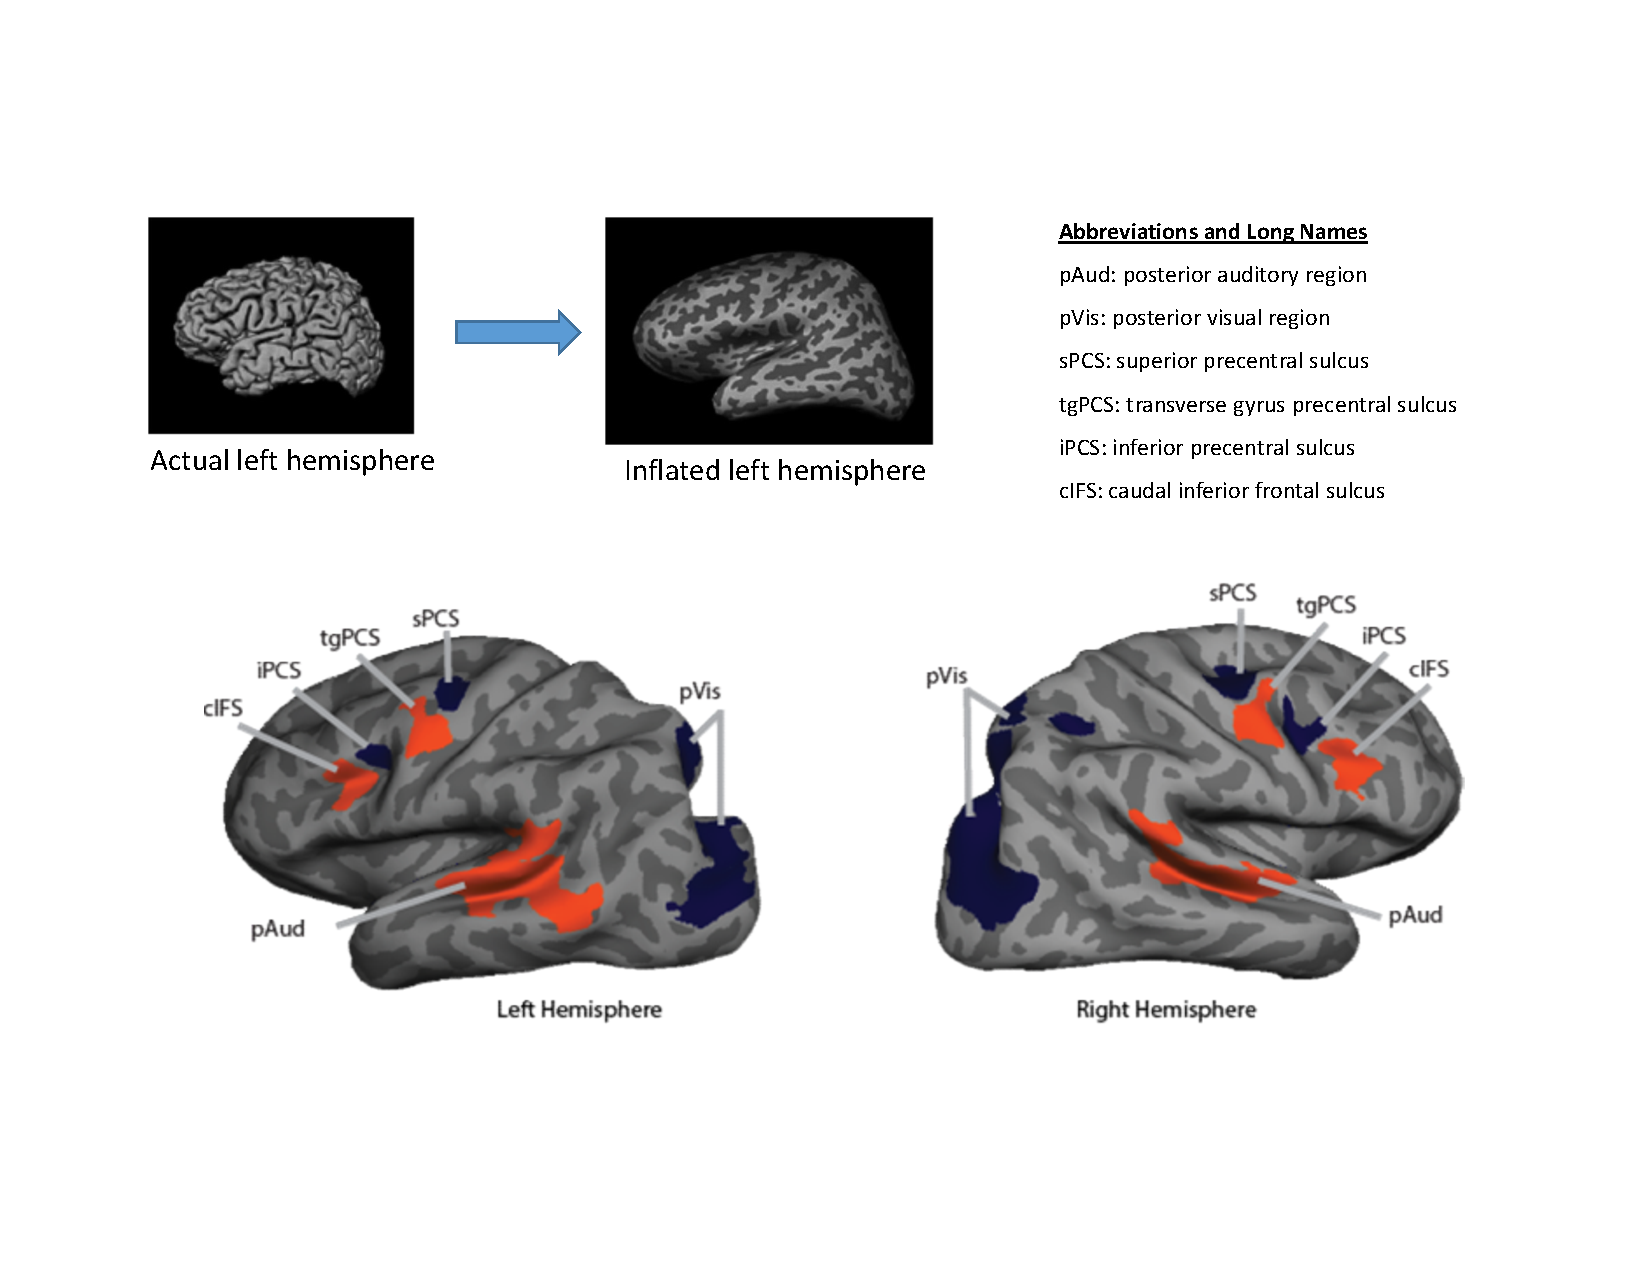
\includegraphics[width=0.75\textwidth]{FacesDay4/figs/brainimages.pdf}
\end{center}

The fundamental idea behind what we are looking for is as follows:
\begin{itemize}
\item The brain can be divided into different regions (physical areas of the brain that are thought to serve some shared purpose). The brain is approximately symmetrical and has a left and a right hemisphere.
\item We have identified 12 brain regions to investigate: 6 in the left hemisphere and 6 in the right hemisphere. They all have long fancy names (such as left superior precentral sulcus) and abbreviations (Left\_sPCS). Due to the symmetry of the brain, there are matching names in each hemisphere (Right\_sPCS and Left\_sPCS both exist).
\item The 12 brain regions that were selected were chosen because a previous experiment indicated that these regions are part of two different networks: one network that is more involved in processing auditory (sound) information and one network that is more involved in processing visual information.
\item Our goal is to look at the correlation between the activity in each of these regions and the other 11 regions. Based on our first study, we hypothesize that the regions in blue will be correlated with other regions in blue to form a ``visual network'' and the regions in orange will be correlated with other regions in orange to form an ``auditory network''.
\end{itemize}
We have given you the data from one person (the actual study had more people). Also, we are not going to worry about statistical testing here; we are just going to look at the correlations in relation to each other.

\begin{center}
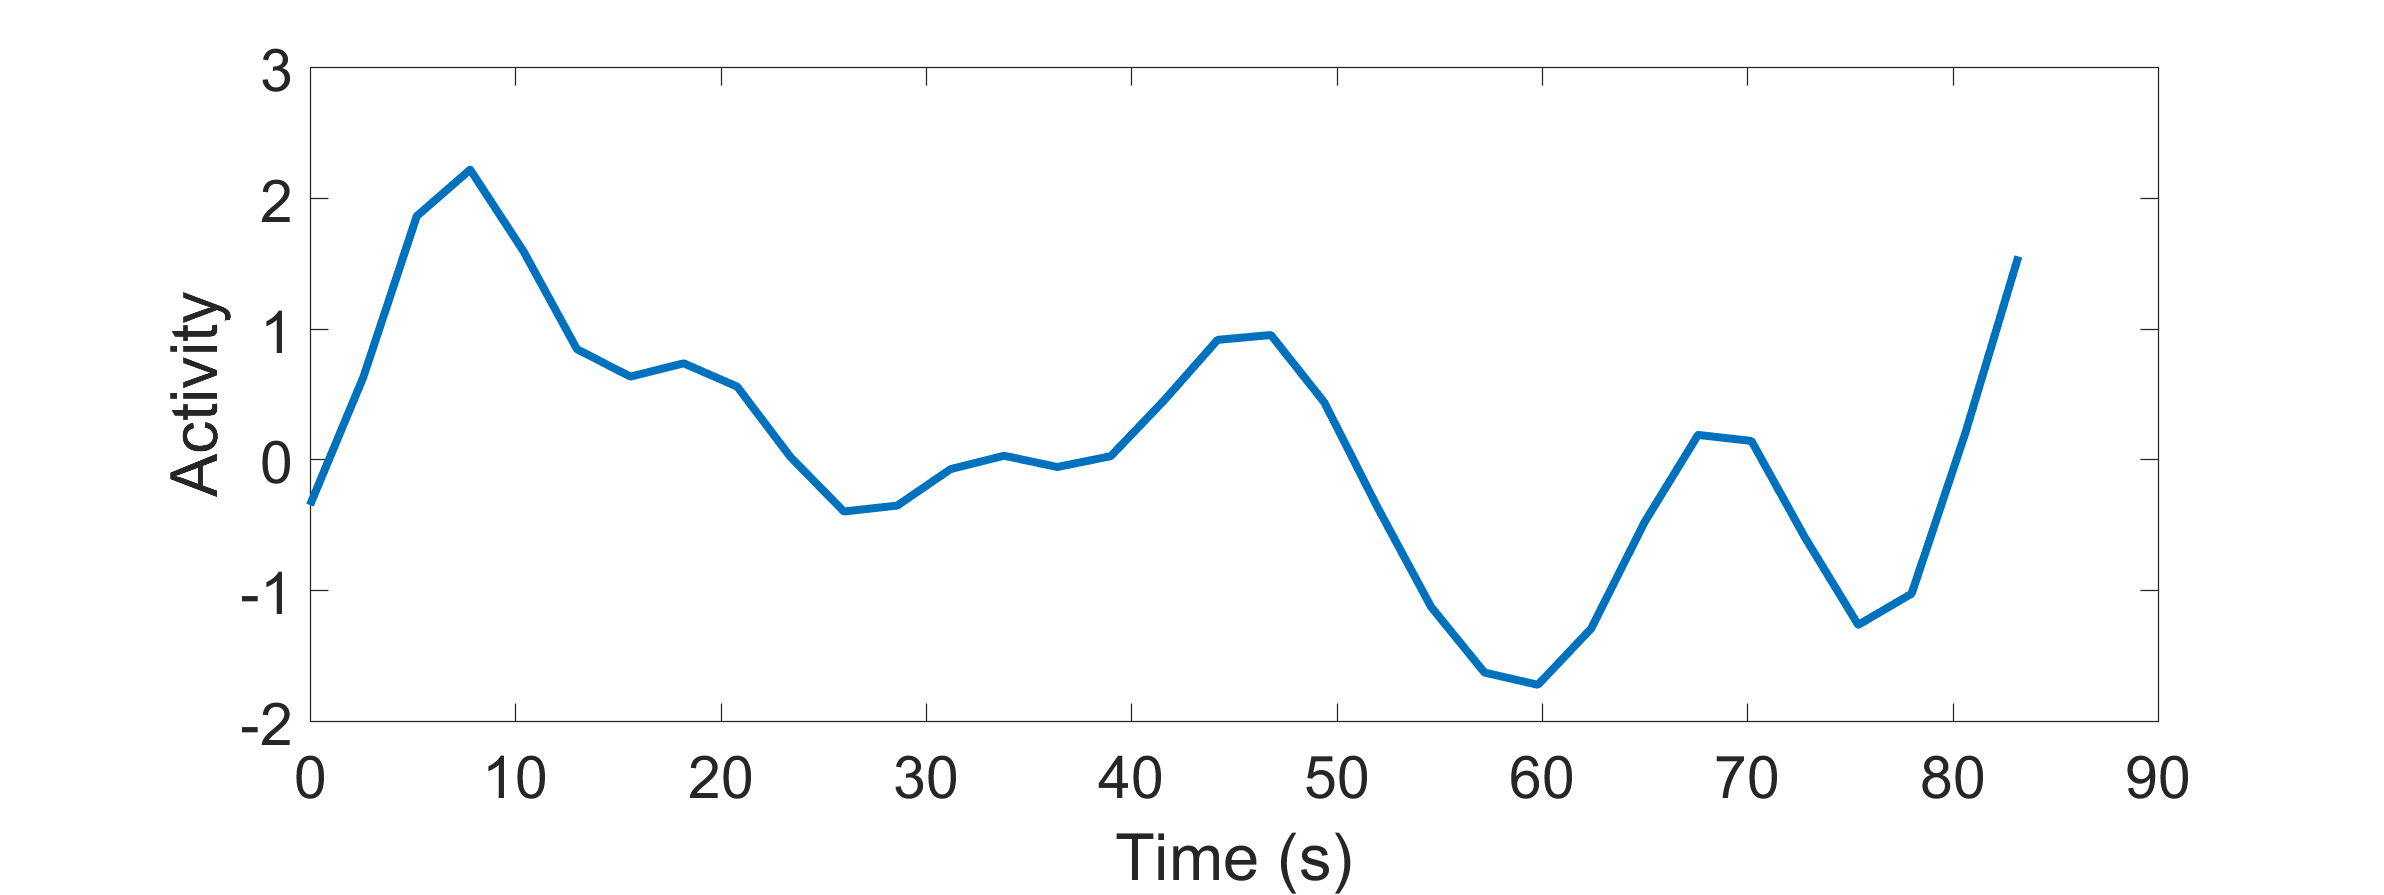
\includegraphics[width=0.75\textwidth]{FacesDay4/figs/brainrpaud80.png}
\end{center}

Let's analyze some brain data! The plot below shows the first 80-ish seconds of data from the ``right posterior auditory region'' or ``Right\_pAud''.

\begin{prob}
\begin{enumerate}
\item \textbf{Consider your data and hypothesis.} Before you transform into a Matlab-mastermind, let's take a minute to think and work on the whiteboard.
\begin{enumerate}
\item Roughly sketch a signal like the one shown in the plot above and label it ``A''.  Don't worry about the details of this signal, just draw some bumps at approximately the same places.
\item Sketch a line for a signal that has a high (but not perfect) positive correlation with ``A''. Label it ``B''. (A different color for each signal would be nice, if convenient.)
\item Sketch a line for a signal that has a high (but not perfect) negative correlation with ``A''. Label it ``C''.
\item Sketch a line for a signal that is uncorrelated with ``A''. Label it ``D''.
\item Make a rough estimate of the correlation between each of these pairs of signals. Organize these estimates in a 4 x 4 table and add labels.
\item Discuss alternate signals that you could have drawn for B, C, and/or D.
\end{enumerate}

\item \textbf{Load and explore the data.} Whenever you encounter a new data set, it's helpful to look at the variables and make a few quick plots.
\begin{enumerate}
	\item Load the fmridata.mat file.
	\item Make sure you have the proper variables.
	\begin{itemize}
		\item There should be 12 brain region vectors, each starting with the word ``Left'' or ``Right'' (e.g., \texttt{Left\_sPCS}). Each value in the vector contains a measurement at a particular point in time. The data were collected for a period of 11 minutes and 5.6 seconds. Measurements were taken every 2.6 seconds.  A timepoint refers to one of those 2.6 second increments. How many timepoints do you expect? Does this match your vector length?
		\item The variable \texttt{braindata} contains all 12 brain region vectors organized into an array with dimensions \texttt{timepoints} $\times$ \texttt{brain regions}.
		\item The variable \texttt{names} contains the names of the 12 brain regions in an order that matches \texttt{braindata}.
		% Validate this by plotting the vector for a random region using the vector variable and by using braindata. These should be identical.
		\item The variable \texttt{uncleandata} is similar to \texttt{braindata} and can be ignored for now.
\end{itemize}

	\item Generate a plot with time on the x-axis and ``activity'' (the data values) on the y-axis. Represent each brain region as a line. You will first need to generate a new vector called \texttt{time} that represents the appropriate time increments (see above). Do your data seem reasonable? How do you know?
	
%	\item Create a separate histogram for each brain region. [Note: you can use \textit{subplot(3,4,plotnumber)} and a \textit{for loop} to generate these histograms without making 12 individual figures.

%	\item What do you observe from this plotting? Do your data seem reasonable? How do you know?
\end{enumerate}


\item \textbf{Focus on a few pairs of regions.} The plot of all brain regions over all time points had a lot of information, so let's zoom in a bit and tie things back to the question at hand. Are the ``auditory'' (orange) regions correlated with other ``auditory'' regions? And are they correlated with the ``visual'' (blue) regions?  Let's use one ``auditory'' regions called \texttt{Left\_pAud} to investigate. The region \texttt{Left\_pAud} is in the left hemisphere of the brain and should be colored orange in the image of the brains above.

\begin{enumerate}
\item Let's begin looking the relationship between \texttt{Left\_pAud} and \texttt{Right\_pAud}.
\item Look at the brain image to determine if \texttt{Right\_pAud} is an ``auditory'' (orange) or ``visual'' (navy blue) type of region. Do you expect the activity of this region to be correlated with \texttt{Left\_pAud}?
\item Plot the signals from these two regions (with time on the x-axis). You may want to zoom in to the first 100 seconds to get another view. Guess the correlation between these regions.
\item Calculate the correlation between between the two regions using the built-in MATLAB function \texttt{corr} (remember, you can get more information on a MATLAB command by typing, for example \texttt{doc corr} or \texttt{help corr} into the MATLAB command prompt).
\item Is this correlation what you expected? How does it fit into our investigation of the correlation between ``auditory'' and ``visual'' regions?

\item Repeat the steps above to look at the relationship between \texttt{Left\_pAud} and \texttt{Left\_sPCS}.
\item Repeat the steps above to look at the relationship between \texttt{Left\_pAud} and \texttt{Left\_tgPCS}.

\end{enumerate}

\item \textbf{Bonus fun: Generalize your analysis to calculate and display the correlations between all pairs of brain regions.} We looked at a few specific pairs of brain regions, but now we want to investigate our hypothesis by looking at all possible pairs of brain regions.
\begin{enumerate}
\item Create a matrix that contains the values of the correlation between each brain region. This is the same idea as the table of correlations that you wrote on the board. (Hint: Use the \texttt{braindata} matrix instead of the individual brain region vectors.) You can confirm that your values are correct by comparing to the correlations that you calculated above.
\item Display this matrix using \texttt{imagesc}. The following code may be helpful in labeling the plot:
\begin{verbatim}
>> colorbar; colormap('jet'); caxis([-1 1]); 
% Set color bar parameters
>> xticks(1:12); xtickangle(-45); xticklabels(names); 
% Label x axis
>> yticks(1:12); yticklabels(names); 
% Label y axis
\end{verbatim}
\item Discuss your observations from this plot. Refer to the figure with the brain image to determine which brain regions are ``auditory'' regions and which are ``visual'' regions? What patterns to you observe about their correlations?
\end{enumerate}


\item \textbf{More Bonus fun: Explore the effects of preprocessing and outliers.} If you have extra time, check out the data in \textit{uncleandata}. This data has the same structure as \textit{braindata}, but contains some ``bad'' time points (208, 209, 210 , 232) caused by a blip in the recording equipment (this is a real problem that people face, though this example is extreme).

\begin{enumerate}
	\item Plot this data versus time. How does this compare to the ``clean'' data from \texttt{braindata}?
	\item Using the \texttt{uncleandata}, recreate the correlation matrix figure that you created using imagesc(), which shows the correlations between each pair of regions.  How does this compare to your original version of this figure? What is important about these differences?
	\item Try to clean the data yourself. There are many possible ways to deal with these ``bad'' timepoints, so you can choose one to investigate. Some options:
	\begin{itemize}
	\item Remove the timepoints completely.
	\item Replace the values at these time points with the mean of the good timepoints.
	\item Replace the values at these time points with a randomly selected value from the good timepoints.
	\item Another strategy of your choosing.
	\end{itemize}
\item Explain which strategy you chose and why. These are decisions that scientists and engineers have to make. There are pros and cons of each. It's really important to consider these and document the analysis decisions that you make.	
\item Discuss with your partner/table or reflect on your own: what are some of the potential ethical implications of "cleaning" data?

\item Plot the activity in all of the brain regions over time for your ``cleaned'' data.
\item Plot the correlation matrix figure for your ``cleaned'' data.
\item What similarities and differences do you observe between the correlation matrix for the ``unclean'' and ``clean'' data? How do you interpret these differences? What do you take away from this for future work?
\end{enumerate}
\end{enumerate}
\end{prob}

\section{AI and Society Discussion}

\subsection{Framing (5 minutes)}

Today we'll be talking about a constellation of issues that arise when AI technology, like facial recognition, is deployed in society.  As the historian Melvin Kranzberg famously remarked, ``Technology is neither good nor bad; nor is it neutral.''  As you saw in the reading from the night assignment, the effect of AI technology in society intersects a number of sensitive issues around race, class, and gender.  Due to intersection of AI and these sensitive issues, it helps to take a few minutes to consider some guidelines for having fruitful discussions at your tables.

\begin{itemize}
\item Check out \href{https://drive.google.com/file/d/1RZ9VHbWvsJwDbyF6zrmkd5mUdINrzt_f/view}{this poster} put together by some Oliners with suggestions for having conversations on sensitive topics.
\item The readings provide common information and framing, which we find is very helpful to finding common ground when discussing issues that individuals may relate to in very different ways.
\item As you may be relatively new to these ideas, consider adopting a mindset of identifying key questions rather than necessarily coming to conclusions.
\item When talking about the effect of a technology on a group that has been historically oppressed, you should be particularly sensitive in these discussions if you are not a member of this group.  Be conscious of the ways in which your words might be experienced by those who may have faced a history of discrimination due to being a member of this group.
\end{itemize}

\subsection{Unpacking the Readings (15 minutes)}
Write down key concepts and clear up points of confusion on the readings.

\begin{itemize}
\item \href{https://docs.house.gov/meetings/GO/GO00/20190522/109521/HHRG-116-GO00-Wstate-BuolamwiniJ-20190522.pdf}{Joy Buolamwini's written testimony} on bias in facial recognition technology (you may have watched this instead).
\item \href{https://www.fatml.org/resources/principles-for-accountable-algorithms}{Principles for Accountable Algorithms}
\item \href{https://cloud.google.com/inclusive-ml/}{Google's Inclusive ML}
\end{itemize}

\subsection{Share Your Positive Application of AI (10 minutes)}
Go around and share the application of AI that you think has the potential for great positive impact on society. Say a little bit about what you learned and how you think it would have a positive impact (e.g., in what ways and for whom).

\subsection{What Did You Take Away? (15 minutes)}

\textbf{Please have one person take notes on this in some electronic format so they can submit it as part of their day survey}

As a table, discuss what you took away from the readings and your discussion thus far.  Here are some dimensions that you might want to explore.
\begin{enumerate}
\item What parts or quotes from the readings were most surprising / impactful to you?
\item Were you surprised by your reaction to reading any of the material (e.g., felt unexpectedly angry, sad, indifferent)?
\item What are the big questions that have been raised for you (these could be things that were already on your radar or new ones entirely)?  These questions could relate to our society as a whole, your role as a citizien within society, your role as an Olin student, your future career path, etc.).
\item How do these readings intersect with knowledge you've gained from other contexts (e.g., in other courses or in your daily life experience)?
\end{enumerate}

\pagebreak
\shipoutAnswer